% Figure from MATH 556 notes, section 37. Compile with the notes preamble.
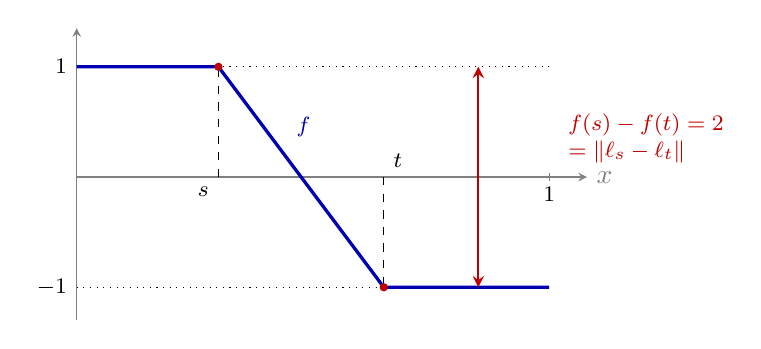
\begin{tikzpicture}[xscale=6, yscale=1.4, >=stealth]
    \draw[->, gray] (0,0) -- (1.08,0) node[right] {$x$};
    \draw[->, gray] (0,-1.3) -- (0,1.35);
    \draw[dotted] (0,1) -- (1,1) (0,-1) -- (1,-1);
    \draw[gray] (1,-0.04) -- (1,0.04);
    \node[left, font=\footnotesize] at (0,1) {$1$};
    \node[left, font=\footnotesize] at (0,-1) {$-1$};
    \node[below, font=\footnotesize] at (1,0) {$1$};
    \draw[very thick, blue!70!black] (0,1) -- (0.3,1) -- (0.65,-1) -- (1,-1);
    \node[blue!70!black, font=\footnotesize] at (0.48,0.45) {$f$};
    \draw[dashed] (0.3,0) -- (0.3,1) (0.65,0) -- (0.65,-1);
    \node[below left, font=\footnotesize] at (0.3,0) {$s$};
    \node[above right, font=\footnotesize] at (0.65,0) {$t$};
    \fill[red!75!black] (0.3,1) circle (0.25pt and 1.07pt);
    \fill[red!75!black] (0.65,-1) circle (0.25pt and 1.07pt);
    \draw[<->, thick, red!75!black] (0.85,1) -- (0.85,-1);
    \node[right, red!75!black, font=\footnotesize, align=left] at (1.02,0.35) {$f(s) - f(t) = 2$\\ $= \|\ell_s - \ell_t\|$};
\end{tikzpicture}
